\question

Un amigo matemático ha propuesto una teoría brillante, que se
representa mediante la siguiente construcción integral:
\begin{equation*}
	\oint
	\kern.15em\vec\varoiintctrclockwise
	\kern-2.60em\varoiintclockwise
\end{equation*}
Ayuda a tu amigo matemático a escribir su teoría y recrear la extraña
integral utilizando los símbolos integrales existentes en Lua\LaTeX.
Consejo: Busca txfonts/pxfonts en symbols-a4 y usa el comando
\mintinline{latex}|\kern| para cambiar el espaciado horizontal.

\begin{solution}
	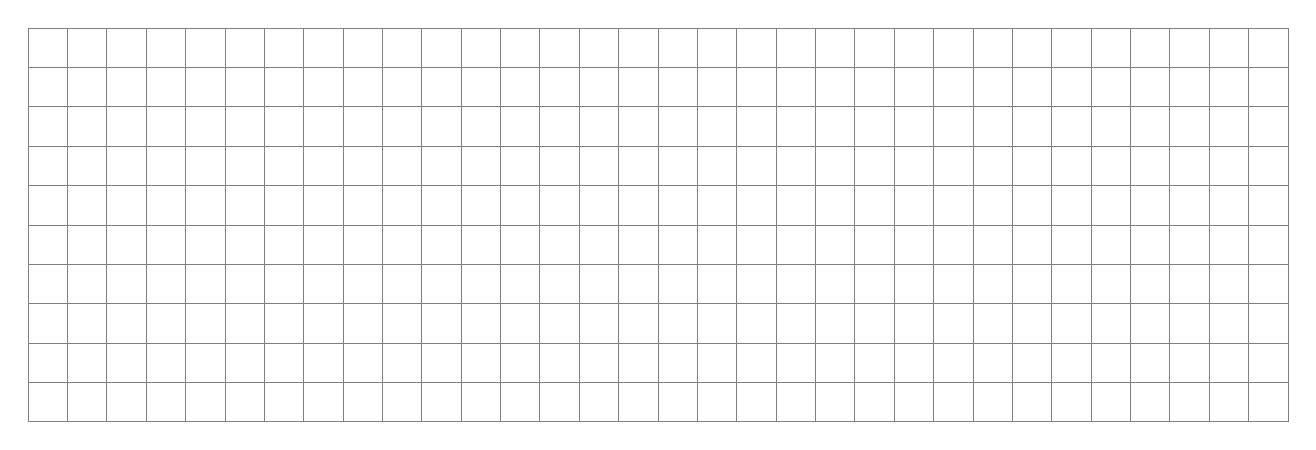
\begin{tikzpicture}[xscale=0.5,yscale=0.5]
		\draw[help lines] (0,0) grid (32,10);
	\end{tikzpicture}
\end{solution}
